\section{Microservice-Steckbrief}
\label{sec: Microservice-Steckbrief}

\begin{figure}[H]
	\begin{center}
	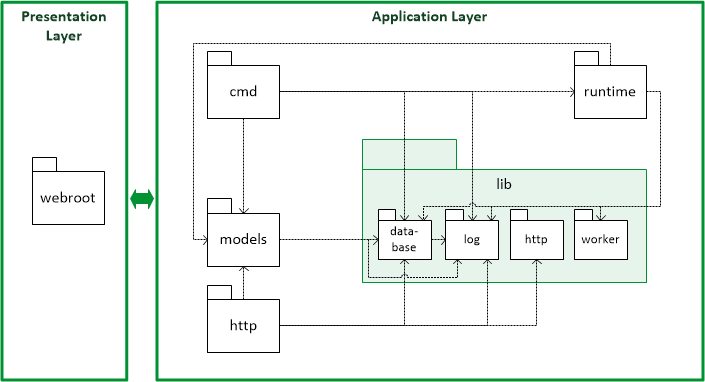
\includegraphics[width=0.65 \textwidth]{./pics/struktur.png}
	\end{center}
	\caption{Microservice Warenwirtschaft}
	\label{pic: Microservice Warenwirtschaft}
\end{figure}


\begin{itemize}
	\item Der Microservice Warenwirtschaft speichert die einzelnen Waren pro Produkt mit ihrem Lagerort und einem Zeitstempel
	\item Das Admin-Frontend erlaubt das Hinzufügen sowie manuelle Löschen von Waren aus dem Warenbestand und zeigt zusätzlich eine Übersicht der Warenbestände
	\item In dem Kunden-Frontend wird der Warenbestand durch ein Ampelsystem dargestellt
	\item Der Microservice wurde in Go entwickelt, die Abbildung \ref{pic: Microservice Warenwirtschaft} gibt einen Überblick der Package-Struktur
	\item Der statische Inhalt der Webseite ist in dem Package \texttt{webroot} verordnet
	\item Als Datenbank wird eine In-Memory-Datenbank im Cache verwendet (Package \texttt{lib})
	\item Die Hauptfunktionalitäten, die zentralen Structs sowie die notwendigen Hilfsfunktionen sind in den Packages \texttt{http} und \texttt{models} verordnet
\end{itemize}
